\documentclass[tikz, border=8pt]{standalone}
\usepackage{amsmath}
\usetikzlibrary{positioning, arrows.meta, calc}

\newcommand{\note}[1]{{\small\itshape #1}}
\newcommand{\boxtitle}[1]{{\bfseries #1}}
\newcommand{\eq}[1]{{\small $#1$}}
\newcommand{\boxgap}{0.9cm}
\newcommand{\derivdrop}{0.6cm}
\newcommand{\topclearance}{0.65cm}
\newcommand{\bottomclearance}{2.45cm}
\newcommand{\eqtight}[1]{{\scriptsize $#1$}}

\begin{document}
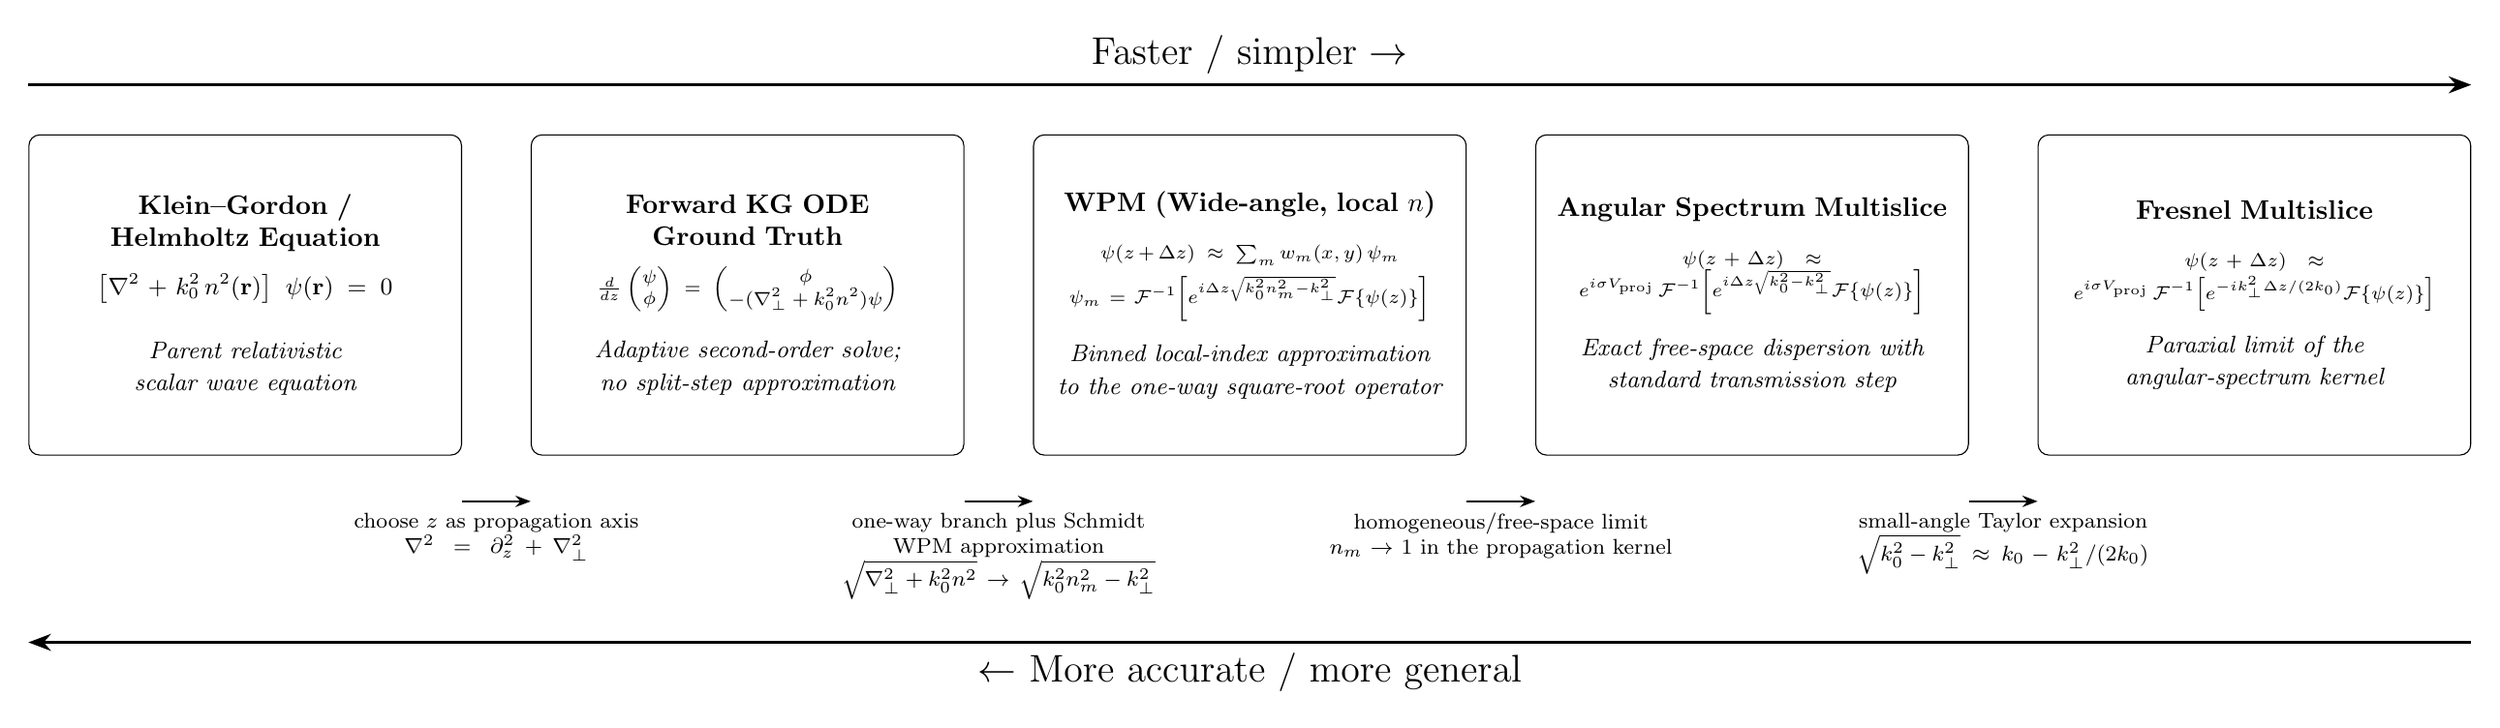
\begin{tikzpicture}[
    box/.style={
        rectangle,
        draw,
        rounded corners,
        align=center,
        text width=5.25cm,
        minimum height=4.2cm,
        inner sep=6pt,
        anchor=center
    },
    deriv/.style={
        align=center,
        font=\footnotesize,
        text width=4.8cm,
        inner sep=2pt
    },
    >=Stealth
]

    % --- 1) Helmholtz / KG equation ---
    \node[box] (helm) {%
        \boxtitle{Klein--Gordon / Helmholtz Equation}\\[6pt]
        \eq{\bigl[\nabla^2 + k_0^2\,n^2(\mathbf{r})\bigr]\;\psi(\mathbf{r})=0}\\[12pt]
        \note{Parent relativistic scalar wave equation}
    };

    % --- 2) Forward KG ODE ground truth ---
    \node[box, right=\boxgap of helm] (ode) {%
        \boxtitle{Forward KG ODE Ground Truth}\\[6pt]
        \eqtight{\frac{d}{dz}\begin{pmatrix}\psi\\\phi\end{pmatrix}=\begin{pmatrix}\phi\\-(\nabla_\perp^2+k_0^2n^2)\psi\end{pmatrix}}\\[10pt]
        \note{Adaptive second-order solve; no split-step approximation}
    };

    % --- 3) WPM (index-dependent spectral step) ---
    \node[box, right=\boxgap of ode] (wpm) {%
        \boxtitle{WPM (Wide-angle, local $n$)}\\[6pt]
        \eqtight{\psi(z\!+\!\Delta z)\approx\sum_m w_m(x,y)\,\psi_m}\\[3pt]
        \eqtight{\psi_m=\mathcal F^{-1}\!\left[e^{i\Delta z\sqrt{k_0^2n_m^2-k_\perp^2}}\mathcal F\{\psi(z)\}\right]}\\[8pt]
        \note{Binned local-index approximation to the one-way square-root operator}
    };

    % --- 4) Angular Spectrum (single homogeneous propagator) ---
    \node[box, right=\boxgap of wpm] (as) {%
        \boxtitle{Angular Spectrum Multislice}\\[6pt]
        \eqtight{\psi(z\!+\!\Delta z)\approx e^{i\sigma V_{\mathrm{proj}}}\,\mathcal F^{-1}\!\left[e^{i\Delta z\sqrt{k_0^2-k_\perp^2}}\mathcal F\{\psi(z)\}\right]}\\[8pt]
        \note{Exact free-space dispersion with standard transmission step}
    };

    % --- 5) Fresnel (paraxial) ---
    \node[box, right=\boxgap of as] (fres) {%
        \boxtitle{Fresnel Multislice}\\[6pt]
        \eqtight{\psi(z\!+\!\Delta z)\approx e^{i\sigma V_{\mathrm{proj}}}\,\mathcal F^{-1}\!\left[e^{-i k_\perp^2\Delta z/(2k_0)}\mathcal F\{\psi(z)\}\right]}\\[8pt]
        \note{Paraxial limit of the angular-spectrum kernel}
    };

    % --- Local derivation annotations between methods ---
    \draw[semithick, ->] ($(helm.south east)+(0,-\derivdrop)$) -- ($(ode.south west)+(0,-\derivdrop)$)
        node[midway, below=2pt, deriv]{choose $z$ as propagation axis\\$\nabla^2=\partial_z^2+\nabla_\perp^2$};

    \draw[semithick, ->] ($(ode.south east)+(0,-\derivdrop)$) -- ($(wpm.south west)+(0,-\derivdrop)$)
        node[midway, below=2pt, deriv]{one-way branch plus Schmidt WPM approximation\\$\sqrt{\nabla_\perp^2+k_0^2n^2}\to\sqrt{k_0^2n_m^2-k_\perp^2}$};

    \draw[semithick, ->] ($(wpm.south east)+(0,-\derivdrop)$) -- ($(as.south west)+(0,-\derivdrop)$)
        node[midway, below=2pt, deriv]{homogeneous/free-space limit\\$n_m\to 1$ in the propagation kernel};

    \draw[semithick, ->] ($(as.south east)+(0,-\derivdrop)$) -- ($(fres.south west)+(0,-\derivdrop)$)
        node[midway, below=2pt, deriv]{small-angle Taylor expansion\\$\sqrt{k_0^2-k_\perp^2}\approx k_0-k_\perp^2/(2k_0)$};

    % --- Tradeoff arrows (top: faster, bottom: more accurate) ---
    % Calculate exact start and end x-coordinates based on bounding boxes
    \coordinate (start_top) at (helm.north west);
    \coordinate (end_top)   at (fres.north east);
    \coordinate (start_bot) at (helm.south west);
    \coordinate (end_bot)   at (fres.south east);

    \draw[very thick, ->] ($(start_top)+(0,\topclearance)$) -- ($(end_top)+(0,\topclearance)$) 
        node[midway, above]{\Large Faster / simpler $\rightarrow$};
    
    \draw[very thick, <-] ($(start_bot)-(0,\bottomclearance)$) -- ($(end_bot)-(0,\bottomclearance)$) 
        node[midway, below]{\Large $\leftarrow$ More accurate / more general};

\end{tikzpicture}
\end{document}